\subsection{UC4 - Modifica della riduzione dimensionale tramite algoritmo}
\begin{figure}[h]
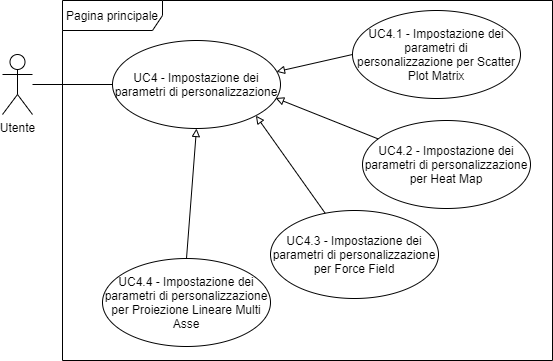
\includegraphics[width=9cm]{Section/Images/UC4.png}
\centering
\caption{UC4 - Modifica della riduzione dimensionale tramite algoritmo}
\end{figure}
\begin{itemize}
	\item \textbf{Attore primario}: Utente;
	\item \textbf{Precondizioni}: L'utente ha scelto l'algoritmo di riduzione dimensionale [UC3.1];
	\item \textbf{Postcondizioni}: I parametri di personalizzazione dell'algoritmo sono stasi impostati e vengono create il numero di dimensioni scelte, pronte per essere visualizzate [UC5];
	\item \textbf{Scenario principale}: L'utente:
	
	\begin{enumerate}
		\item Seleziona il numero di dimensioni da ricavare dalla riduzione dimensionale [UC4.1];
		\item Personalizza i parametri dell'algoritmo di riduzione dimensionale selezionato secondo le sue esigenze [UC4.2].
		\item Imposta il nome che desidera dare alle nuove dimensioni da generare [UC4.3]
	\end{enumerate}		
\end{itemize}

\subsubsection{UC4.1 - Selezione del numero di dimensioni}

\begin{itemize}
	\item \textbf{Attore primario}: Utente;
	
	\item \textbf{Precondizioni}: L'utente ha scelto un algoritmo di riduzione dimensionale [UC3.1];
	
	\item \textbf{Postcondizioni}: L'utente ha selezionato il numero di dimensioni che vuole ottenere dal processo di riduzione dimensionale;
	
	\item \textbf{Scenario principale}: L'utente decide il numero di dimensioni da ricavare selezionando un numero tra l'intervallo disponibile.
\end{itemize}	
	
\newpage	
	
\subsubsection{UC4.2 - Impostazione dei parametri dell'algoritmo}
\begin{figure}[h]
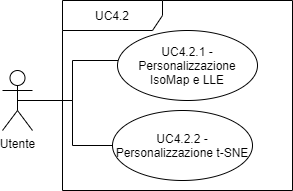
\includegraphics[width=9cm]{Section/Images/UC4.2.png}
\centering
\caption{UC4.2 - Impostazione dei parametri dell'algoritmo}
\end{figure}
\begin{itemize}
	\item \textbf{Attore primario}: Utente;
	
	\item \textbf{Precondizioni}: L'utente ha scelto un algoritmo di riduzione dimensionale [UC3.1];
	
	\item \textbf{Postcondizioni}: L'utente ha impostato i parametri personalizzabili dell'algoritmo;
	
	\item \textbf{Scenario principale}: L'utente imposta i parametri specifici dell'algoritmo selezionato.
	
		\item \textbf{Generalizzazioni}: L'utente imposta i parametri di personalizzazione dell'algoritmo scelto:
	\begin{enumerate}[(a)]
		\item Personalizzazione \glo{\textit{IsoMap}} e \glo{\textit{LLE}} [UC4.2.1];
		\item Personalizzazione \glo{\textit{t-SNE}} [UC4.2.2];
	\end{enumerate}
\end{itemize}		
		

\subsubsection{UC4.2.1 - Personalizzazione IsoMap e LLE}
\begin{itemize}
	\item \textbf{Attore primario}: Utente;
	
	\item \textbf{Precondizioni}: L'utente ha scelto l'algoritmo \textit{IsoMap} [UC3.1.1] oppure \textit{LLE} [UC3.1.2];
	
	\item \textbf{Postcondizioni}: L'algoritmo viene impostato con le personalizzazioni dell'utente;
	
	\item \textbf{Scenario principale}: L'utente seleziona il numero di punti vicini (\glo{\textit{neighbors}}), tra l'intervallo disponibile, per la stima approssimativa del \glo{\textit{manifold}}.

\end{itemize}

\newpage

\subsubsection{UC4.2.2 - Personalizzazione t-SNE}
\begin{figure}[h]
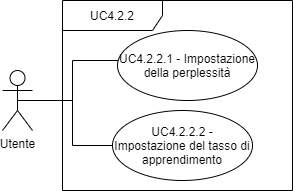
\includegraphics[width=9cm]{Section/Images/UC4.2.2.png}
\centering
\caption{UC4.2.2 - Personalizzazione t-SNE}
\end{figure}
\begin{itemize}
	\item \textbf{Attore primario}: Utente;
	
	\item \textbf{Precondizioni}: L'utente ha scelto l'algoritmo \textit{t-SNE} [UC3.1.4];
	
	\item \textbf{Postcondizioni}: L'algoritmo viene impostato con le personalizzazioni dell'utente;
	
	\item \textbf{Scenario principale}: L'utente decide:

\begin{enumerate}
\item Impostazione della perplessità [UC4.2.2.1];
\item Impostazione del tasso di apprendimento (\glo{\textit{Epsilon}}) [UC4.2.2.2];
\end{enumerate}	

\end{itemize}
	
	
\paragraph{UC4.2.2.1 - Impostazione della perplessità}
\begin{itemize}
	\item \textbf{Attore primario}: Utente;
	
	\item \textbf{Precondizioni}: L'utente ha scelto l'algoritmo \textit{t-SNE} [UC3.1.4];
	
	\item \textbf{Postcondizioni}: L'algoritmo viene impostato con le personalizzazioni dell'utente;
	
	\item \textbf{Scenario principale}: L'utente imposta il valore, tra l'intervallo disponibile, per bilanciare gli aspetti globali e locali dei dati.

\end{itemize}
	
\paragraph{UC4.2.2.2 - Impostazione del tasso di apprendimento}
\begin{itemize}
	\item \textbf{Attore primario}: Utente;
	
	\item \textbf{Precondizioni}: L'utente ha scelto l'algoritmo \textit{t-SNE} [UC3.1.4];
	
	\item \textbf{Postcondizioni}: L'algoritmo viene impostato con le personalizzazioni dell'utente;
	
	\item \textbf{Scenario principale}: L'utente imposta il valore, tra l'intervallo disponibile, del tasso di apprendimento dell'algoritmo.

\end{itemize}

\subsubsection{UC4.3 - Assegnazione del nome alle dimensioni create}

\begin{itemize}
	\item \textbf{Attore primario}: Utente;
	
	\item \textbf{Precondizioni}: L'utente ha scelto un algoritmo di riduzione dimensionale [UC3.1];
	
	\item \textbf{Postcondizioni}: L'utente ha assegnato i nomi alle dimensioni che andrà a creare;
	
	\item \textbf{Scenario principale}: L'utente assegna il nome alle dimensioni che sta creando nell'apposito campo d'input; il nome scelto sarà seguito da un numero crescente, che dipende dal numero di dimensioni generate. Se non modificato vengono mantenuti i nomi di default, costituiti dal nome dell'algoritmo scelto.

\end{itemize}	
